\chapter{Architecture Study}\label{Study1}

The primary objective of this study is to evaluate how well different neural network architectures perform on the task of \acrfull{ADT}, with a specific focus on \acrfull{DTM}. The goal is to identify which architectures are most effective for this task, to observe possible common patterns among high-performing models, and to determine whether certain architectural designs consistently underperform. These findings will help assess which architectures are best suited for complex \gls{ADT} tasks and how architecture choice may influence a model's ability to generalize.

\section{Methodology}

To effectively assess the strengths and weaknesses of each architecture within-domain across all datasets, I conduct an experiment for each architecture/dataset combination. For each combination, I train multiple models (either 15 or 25) and select the best-performing one based on validation performance. The selected model is then evaluated on the test split of the same dataset it was trained on. As a result, all reported performance metrics reflect performance on unseen data drawn from the same distribution as the training set. 

Each model is trained and validated exclusively on one dataset, and evaluated only on its corresponding test set. This approach provides insight into each architecture's ability to learn the \gls{ADT} task and serves as a basis for comparing their generalization performance within-domain.

\section{Results}	

\begin{table}[H]
    \centering
    \hspace*{-0.6cm}
    \begin{tabular}{l|cccc}
        Architecture & ENST+MDB & E-GMD & Slakh & ADTOF-YT       \\
        \hline
        Recurrent Neural Network	& 0.67 &	\textbf{0.90} &	0.86 &	\textbf{0.96} \\
        Convolutional Neural Network	& 0.78 &	0.88 &	0.83 &	0.84 \\
        Convolutional Recurrent Neural Network	& \textbf{0.81} &	\textbf{0.90} &	\textbf{0.90} &	0.93 \\
        Convolutional Transformer	& 0.77 & 0.89 &	0.88 &	0.95 \\
        Vision Transformer	& 0.54 &	0.89 &	0.88 &	\textbf{0.96} \\
        
    \end{tabular}
    \caption{Test micro F1-score for each architecture, trained and evaluated on splits of the same dataset. \textbf{Bold} values represent the highest score achieved for that dataset.}
    \label{ArchitectureResultsTable}
\end{table}


\begin{figure}[H]
    \centering
    \hspace*{-0.8cm}
    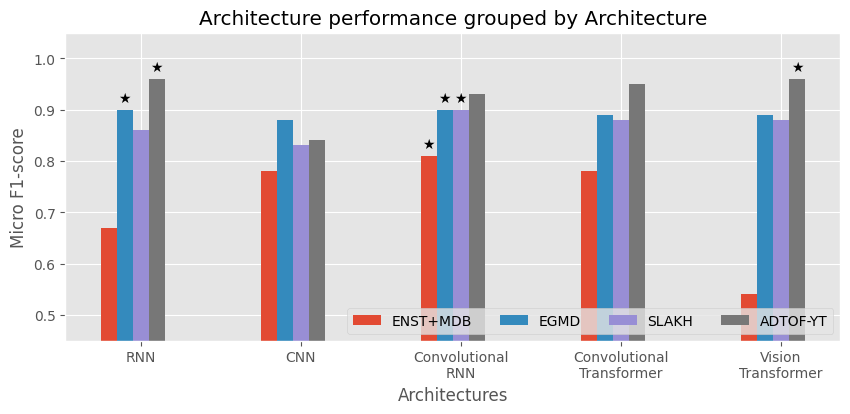
\includegraphics[scale=0.8]{figures/architectureperformancearchitecture.png}
    \caption{Test micro F1-scores per dataset, grouped by architecture. Bars marked with a ($\star$) indicate the best-performing architecture for each dataset.}
    \label{ArchitectureResultsArchitectureFigure}
\end{figure}

\begin{figure}[H]
    \centering
    \hspace*{-0.8cm}
    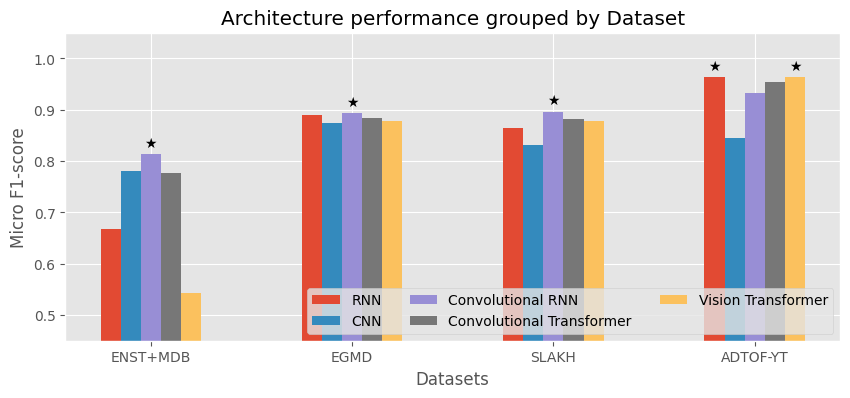
\includegraphics[scale=0.8]{figures/architectureperformancedataset.png}
    \caption{Test micro F1-scores per architecture, grouped by dataset. Bars marked with a ($\star$) indicate the best-performing architecture for each dataset.}
    \label{ArchitectureResultsDatasetFigure}
\end{figure}

\begin{figure}[H]
    \centering
    \begin{tikzpicture}
    \matrix[label=north:{\acrshort{CRNN} — ENST+MDB Sample}] {
        \node[label=west:{Target Sequence}] {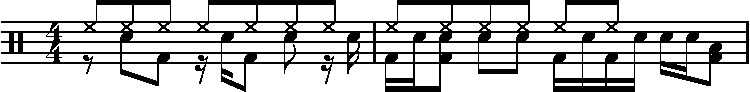
\includegraphics[scale=1.0]{lilypond/predictions/enst+mdb.cropped.pdf}}; \\
        \node[label=west:{Predicted Sequence}] {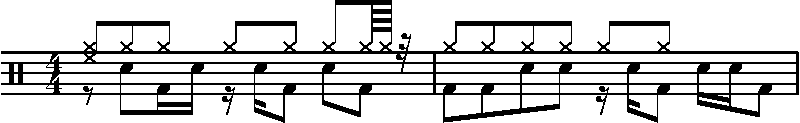
\includegraphics[scale=0.94]{lilypond/predictions/enst+mdb_prediction.cropped.pdf}}; \\};
    \end{tikzpicture}
    \caption{Prediction example from the \acrfull{CRNN} on a randomly selected sequence from the ENST+MDB test split. This is a complex drum pattern, but the transcription is generally accurate. Most onsets are correctly placed and labeled, although several \acrfullpl{FP} and \acrfullpl{FN} occur.}
    \label{ArchitecturePredictionComparisonENST+MDBFigure}
\end{figure}

\begin{figure}[H]
    \centering
    \begin{tikzpicture}
    \matrix[label=north:{\acrshort{CRNN} — E-GMD Sample}] {
        \node[label=west:{Target Sequence}] {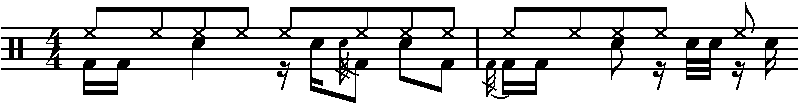
\includegraphics[scale=0.9]{lilypond/predictions/egmd.cropped.pdf}}; \\
        \node[label=west:{Predicted Sequence}] {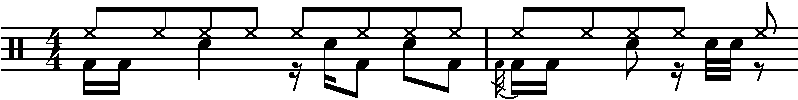
\includegraphics[scale=0.9]{lilypond/predictions/egmd_prediction.cropped.pdf}}; \\};
    \end{tikzpicture}
    \caption{Prediction example from the \acrfull{CRNN} on a randomly selected sequence from the E-GMD test split. The drum pattern is moderately complex, but the model transcribed it with high accuracy. Only two \acrfullpl{FN} are present, and the prediction aligns closely with the target sequence. Note that E-GMD is a \gls{DTD} dataset without melodic accompaniment, which may make the transcription task slightly easier.}
    \label{ArchitecturePredictionComparisonEGMDFigure}
\end{figure}

\begin{figure}[H]
    \centering
    \begin{tikzpicture}
    \matrix[label=north:{\acrshort{CRNN} — Slakh Sample}] {
        \node[label=west:{Target Sequence}] {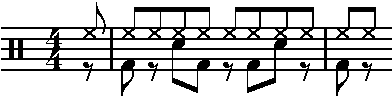
\includegraphics[scale=1.2]{lilypond/predictions/slakh.cropped.pdf}}; \\
        \node[label=west:{Predicted Sequence}] {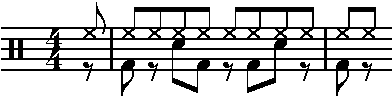
\includegraphics[scale=1.2]{lilypond/predictions/slakh_prediction.cropped.pdf}}; \\};
    \end{tikzpicture}
    \caption{Prediction example from the \acrfull{CRNN} on a randomly selected sequence from the Slakh test split. The drum pattern is relatively simple, and the model produces a perfect transcription with all onsets correctly placed and labeled.}
    \label{ArchitecturePredictionComparisonSlakhFigure}
\end{figure}

\begin{figure}[H]
    \centering
    \begin{tikzpicture}
    \matrix[label=north:{\acrshort{CRNN} — ADTOF-YT Sample}] {
        \node[label=west:{Target Sequence}] {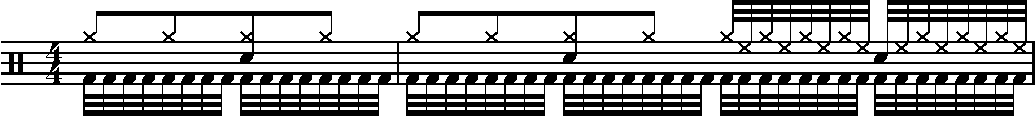
\includegraphics[scale=0.7]{lilypond/predictions/adtof_yt.cropped.pdf}}; \\
        \node[label=west:{Predicted Sequence}] {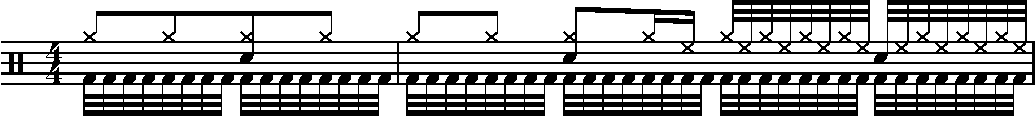
\includegraphics[scale=0.7]{lilypond/predictions/adtof_yt_prediction.cropped.pdf}}; \\};
    \end{tikzpicture}
    \caption{Prediction example from the \acrfull{CRNN} on a randomly selected sequence from the ADTOF-YT test split. The pattern is dense, originating from a metal track, yet the model performs remarkably well. Only a single \acrfull{FP} is present, with all other onsets accurately transcribed.}
    \label{ArchitecturePredictionComparisonADTOF-YTFigure}
\end{figure}

\section{Discussion}

The results from the architecture study, summarized in Table~\ref{ArchitectureResultsTable} and Figures~\ref{ArchitectureResultsArchitectureFigure} and~\ref{ArchitectureResultsDatasetFigure}, indicate that there is no single architecture that consistently outperforms the others for \gls{ADT}. Instead, performance varies depending on the characteristics of each dataset and the inductive biases inherent to each architectural design.

Firstly, while multiple architectures perform well across different datasets, none emerge as universally superiour. No single architecture consistently outperforms the others on all the datasets, several architectures exhibit similarly strong results depending on the dataset. 

However, the convolutional recurrent neural network demonstrates the highest micro F1-score on three of the four datasets (namely ENST+MDB, E-GMD and Slakh). It also performs strongly, but not exceptionally, on the fourth (ADTOF-YT). The consistency of its high performance across datasets with differing characteristics suggests that it is capable of handling a wide variety of \gls{ADT} tasks. This robustness appears to hold relatively independently of dataset size or complexity. 

One possible explanation for this is the architectural synergy between the convolutional and recurrent layers. The convolutional blocks provide a strong spatial feature extraction over local time–frequency patches, while the recurrent layers enable short-range temporal modeling. Together, these inductive biases may make the \gls{CRNN} especially well-suited for the challenges of \gls{ADT}.

--

The convolutional neural network displays a moderate performance across all datasets. It shows adequate performance on the smallest dataset (ENST+MDB), having the second highest F1-score. However, across all others (E-GMD, Slakh and ADTOF-YT) it displays the lowest. This relatively poor overall performance seems to indicate that the convolutional neural network currently is an inferior architecture for \gls{ADT} tasks, unless dataset size is limited, in which it could provide a viable architecture. It also shows the importance of explicitly leveraging the temporal dependencies within \gls{ADT}, as solely relying on the inductive bias of the convolutions didn't prove sufficient here.

This importance seems to be strengthened by the performance of the purely recurrent neural network, which has a surprisingly high performance across the datasets. In a way, it displays the opposite behaviour compared to the \gls{CNN}, displaying inadequate performance for the smallest dataset (ENST+MDB), but a relatively high performance for two of the others (E-GMD and Slakh), sharing the crown for the highest F1-score on the last (ADTOF-YT). The first dataset's low performance suggests that the inductive bias of the recurrent layers are "weaker" than the ones from convolutions, relying on a larger amount of data to accurately learn the task. Notably, it significantly outperforms the \gls{CRNN} on the last dataset, hinting that the inductive bias of the convolutions might "overpower" the model, proving so strong that it ends up hindering its performance.

The convolutional transformers exhibits performance comparable to something in between the \gls{RNN} and \gls{CRNN}, and shows what can be described as the most consistent relatively high performance across all the four datasets. It puts itself just under the \gls{CRNN} for the first three datasets (ENST+MDB, E-GMD and Slakh), and a good step over for the last (ADTOF-YT). This does seem to indicate that the transformer models provide enough of a temporal inductive bias to accurately perform well on \gls{ADT} tasks, however it might also hint that the long range dependencies more easily modelled with attention layers are not as important as the accurate short range aggregation from the recurrent layers on most \gls{ADT} datasets. Although by the performance displayed, the convolutional transformer could be chosen as a viable architecture for \gls{ADT}.

At last we have the Vision transformer, which performs similar to the \gls{RNN}. For the smallest dataset (ENST+MDB) it displays a subpar performance with by far the lowest F1-score. For the two middle ones (E-GMD and Slakh) it exhibits a relatively average performance. For the last dataset (ADTOF-YT) it shows excellent performance, having an identical F1-score to the \gls{RNN}. This seems to agree with the previous conclusion that the inductive bias of the convolutional layers are "strong", putting a higher responsibility on a large amount of quality data when omitting it. The significantly poor performance on the small dataset might also indicate that the attention layers and transformer blocks come with an even "weaker" inductive bias than the recurrent layers, hightening the reliance on data amount. This aligns well with existing literature, where vision transformers generally require extensive training data or pre-training on larger datasets to obtain optimal performance~\cite{dosovitskiy2021imageworth16x16words}.

In summary, our results strongly indicate that the Convolutional Recurrent Neural Network is the current most suited architecture for \gls{ADT} tasks across different datasets. However, further research should be done into both the Vision Transformer and Recurrent Neural Network, gauging how these models scale with larger datasets.

\textcolor{red}{Is it relevant to talk about future research here or should it be in the final conclusion?}